\subsection {Session 11, Exercise 11}

\lineparagraph {Exercise}

Vertices of a binary tree are labeled by integers between $0$ and $9$ (inclusive). The $InOrder$ walk lists the
labels as $9, 3, 1, 0, 4, 2, 7, 6, 8, 5$, while the PostOrder lists them as $9, 1, 4, 0, 3, x, 7, 5, y, 2$. What could
$x$ and $y$ be?


\lineparagraph {Solution}

\begin{itemize}
    \item Note here: \textbf{the labels are not the keys} based on which the binary tree is structured! We can see this since the $InOrder$ walk is supposed to return the keys in increasing order and the labels it returned are not sorted!
    \item The labels are just there to hide the actual keys from you in this exercise.
    \item First let's talk about the $PreOrder$, $InOrder$ and $PostOrder$, walks of the binary search tree:
    \item Let's imagine that the following struct represent a node in the tree:
\end{itemize}

\begin{minted}[linenos]{c++}
struct {
    int key;
    node* left;
    node* right;
} node;
\end{minted}

\begin{itemize}
    \item Now, every single walk will explore the left-side of any node first and the right-side later. The difference comes from \textbf{when the current node itself is explored}.
\end{itemize}

\begin{minted}[linenos]{c++}
void preOrder(node current) {
  // Explores current node before moving on to children.
  cout << current.key;
  preOrder(current->left);
  preOrder(current->right);
}

void inOrder(node current) {
  inOrder(current->left);
  // Explores current node after finishing left but before starting right child.
  cout << current.key;
  inOrder(current->right);
}

void postOrder(node current) {
  postOrder(current->left);
  postOrder(current->right);
  // Explores current node after all children were explored.
  cout << current.key;
}
\end{minted}

\begin{itemize}
    \item Let's run these algorithms on an example:
\end{itemize}

\begin{center}
    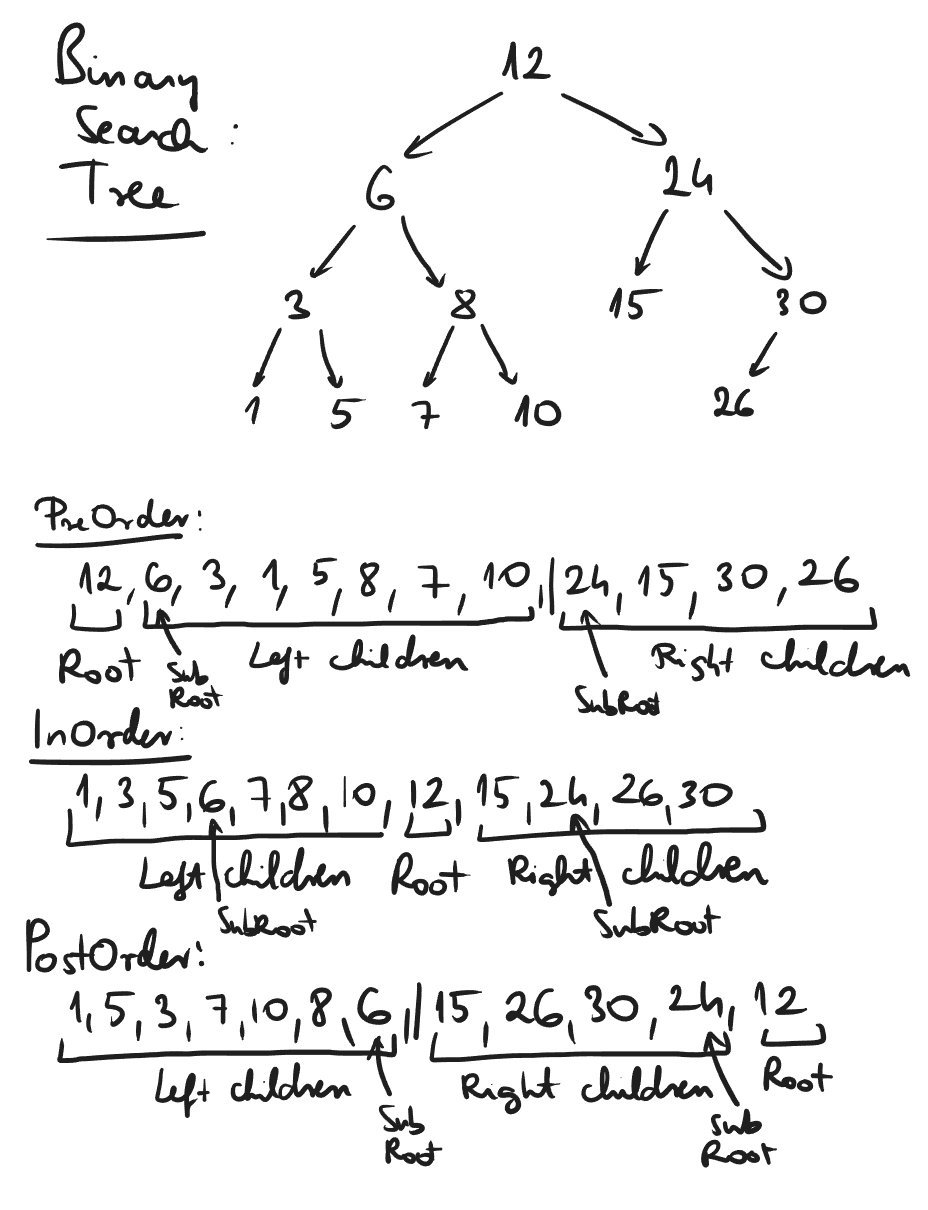
\includegraphics[width=\linewidth]{11/11/bst_walks.png}
\end{center}

\begin{itemize}
    \item Interestingly, if we are given the InOrder walk result and either a PostOrder or a PreOrder result, we will be able to reconstruct the original tree.
    \item In this example, the InOrder result is redundant, since we know the correct increasing order of the number, but in the case of the original exercise the labels hide this information.
    \item So let's say if we know the InOrder and PostOrder results:
    \item At first, we look at the PostOrder result. We know for a fact, that the Root of the entire tree will be the very last element in this result.
    \item So looking at the PostOrder numbers, we know that the root is $12$.
    \item Now we look over to the InOrder list: here the Root is going to be between its left children and right children.
    \item From this information we know that the left children of $12$ are $1,3,5,6,7,8,10$ and the right children are $15,24,26,30$.
    \item Now if we look back at the PostOrder results, we finally know that the separator between the left and right children is actually between $6$ and $15$.
    \item We can now continue the same thing recursively for the two subtrees.
    \item The root of the left subtree is $6$, since that is the last element of that subtree in the PostOrder result.
    \item If we look at the InOrder result for that subtree, we know that $6$ is between its left and right children, so the left children of $6$ must be $1,3,5$ and the right children must be $7,8,10$.
    \item You can try to finish this example at home, but I will do this algorithm for the original exercise.
\end{itemize}


\begin{center}
    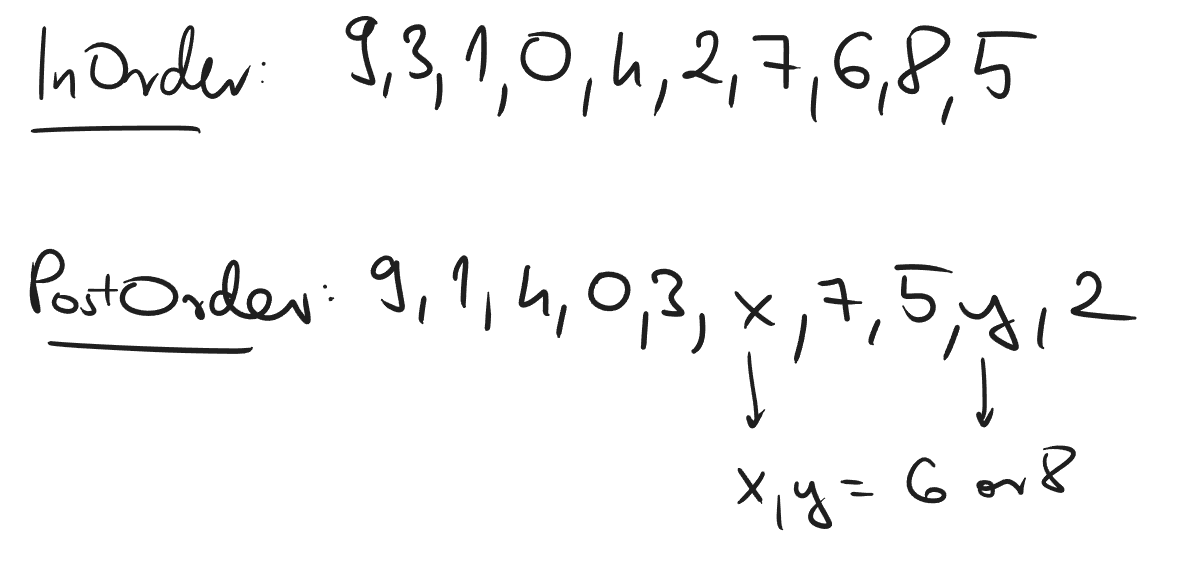
\includegraphics[width=\linewidth]{11/11/reconstruct_01.png}
\end{center}

\begin{itemize}
    \item We see that the two missing numbers from the PostOrder walk are $6$ and $8$ so $x$ and $y$ will be these two in some order.
\end{itemize}


\begin{center}
    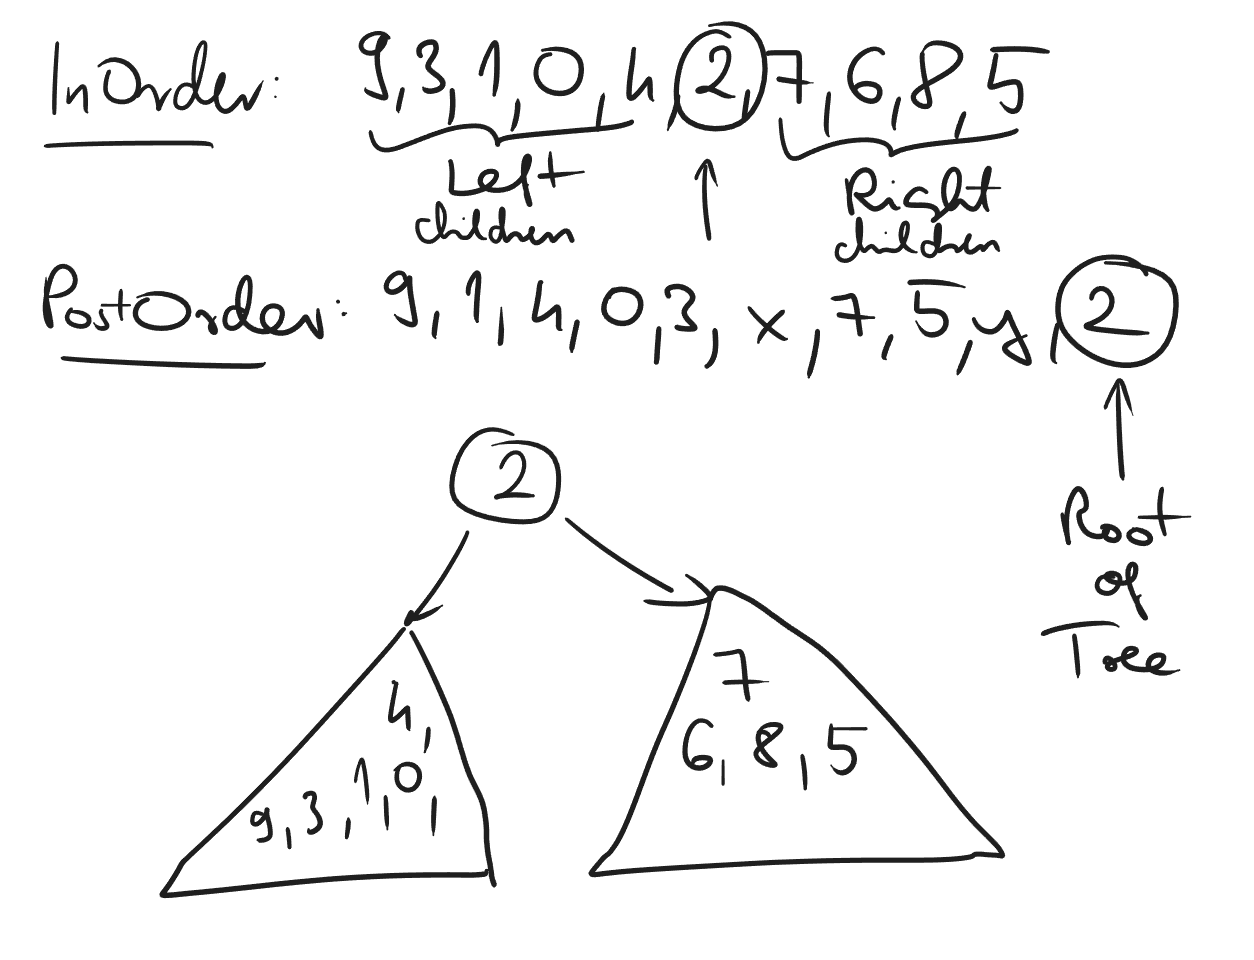
\includegraphics[width=\linewidth]{11/11/reconstruct_02.png}
\end{center}

\begin{itemize}
    \item Since $2$ is the last element of the PostOrder walk, that is the root of the tree.
    \item Looking at the InOrder result, we see which elements are on its left and which are on its right.
\end{itemize}


\begin{center}
    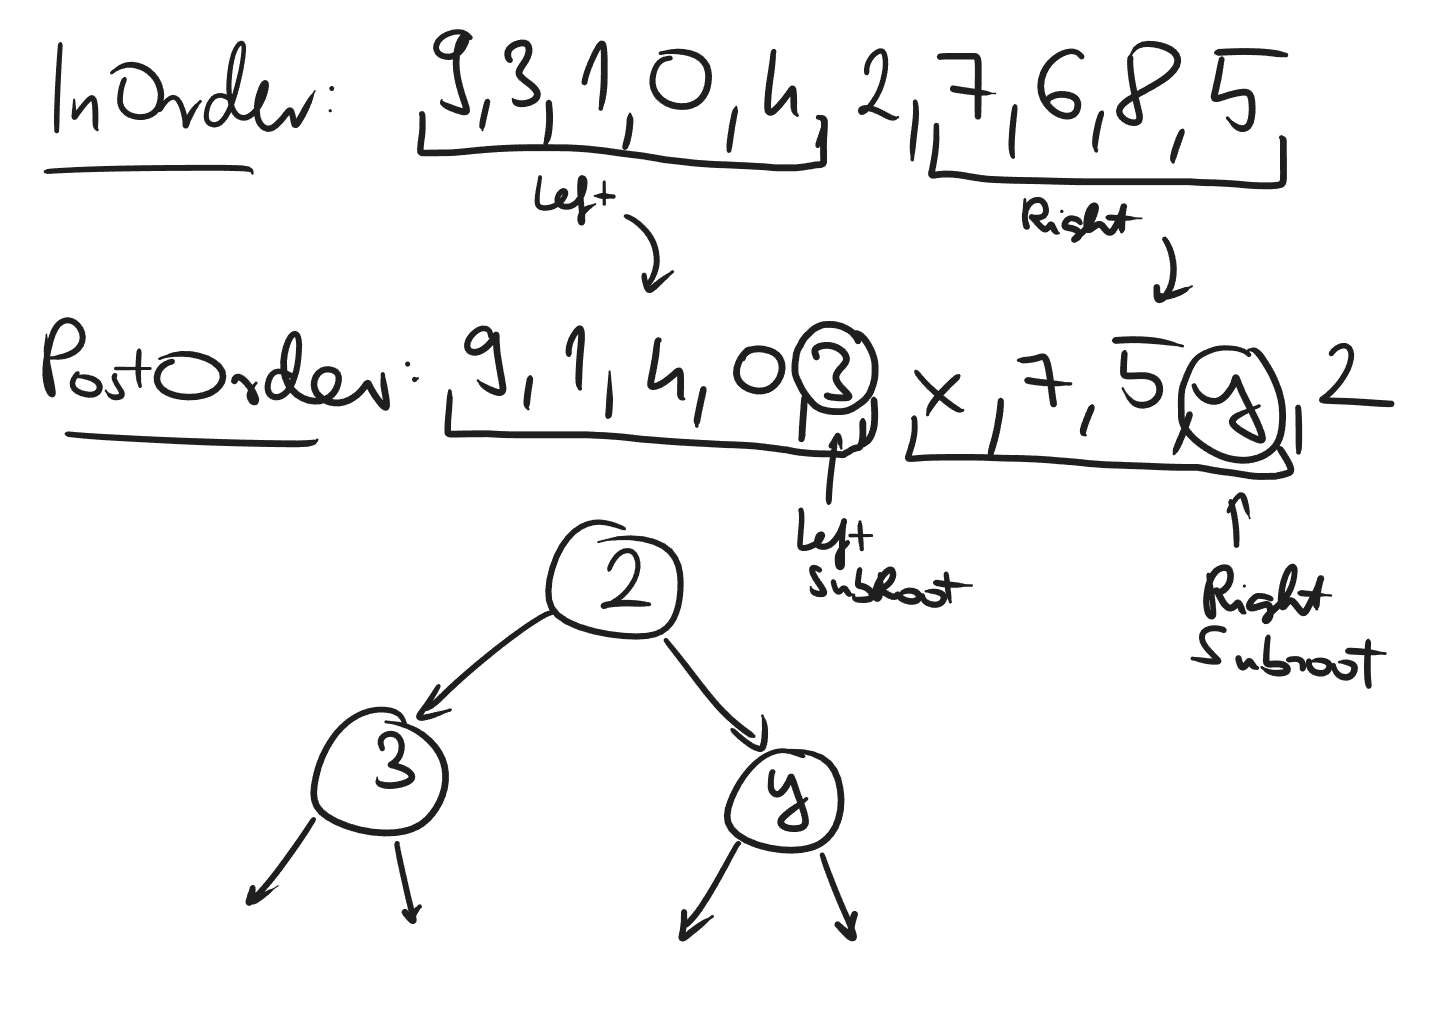
\includegraphics[width=\linewidth]{11/11/reconstruct_03.png}
\end{center}

\begin{itemize}
    \item If we go back to the PostOrder result and look for the same elements, we see that the subroot of the tree on the left is $3$, since that is the last element of that sublist. Similarly, $y$ is the root of the right subtree, since that is the last element of that sublist. Both $x$ and $y$ must be on the righthand side of the root.
\end{itemize}

\begin{center}
    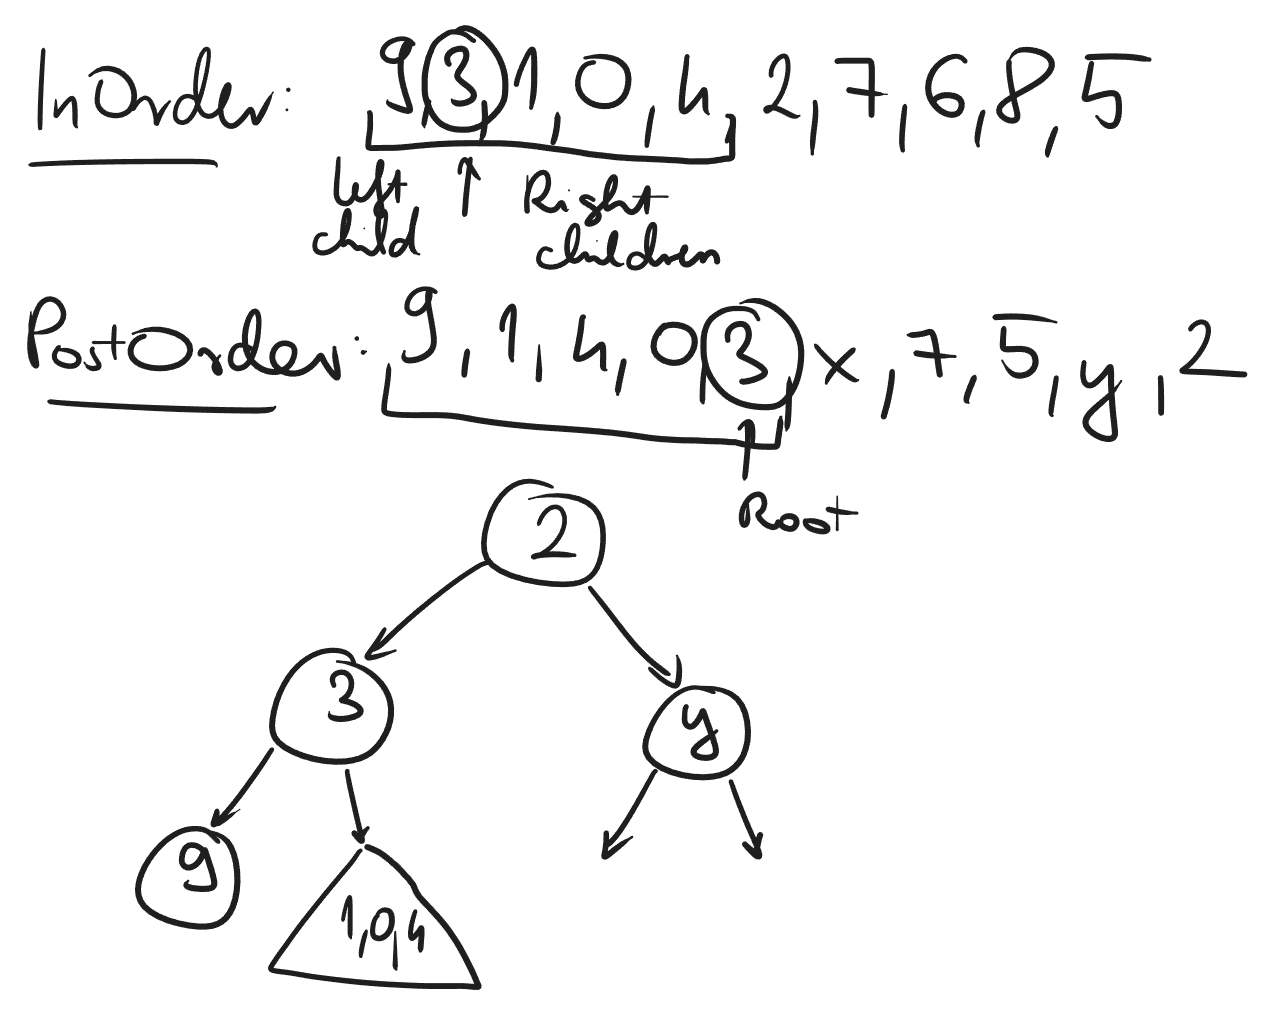
\includegraphics[width=\linewidth]{11/11/reconstruct_04.png}
\end{center}

\begin{itemize}
    \item If we continue on the left side, we see that the root is $3$, so looking at the InOrder list, we see that the left child is just the number $9$, while the right side contains numbers $1,0,4$.
\end{itemize}

\begin{center}
    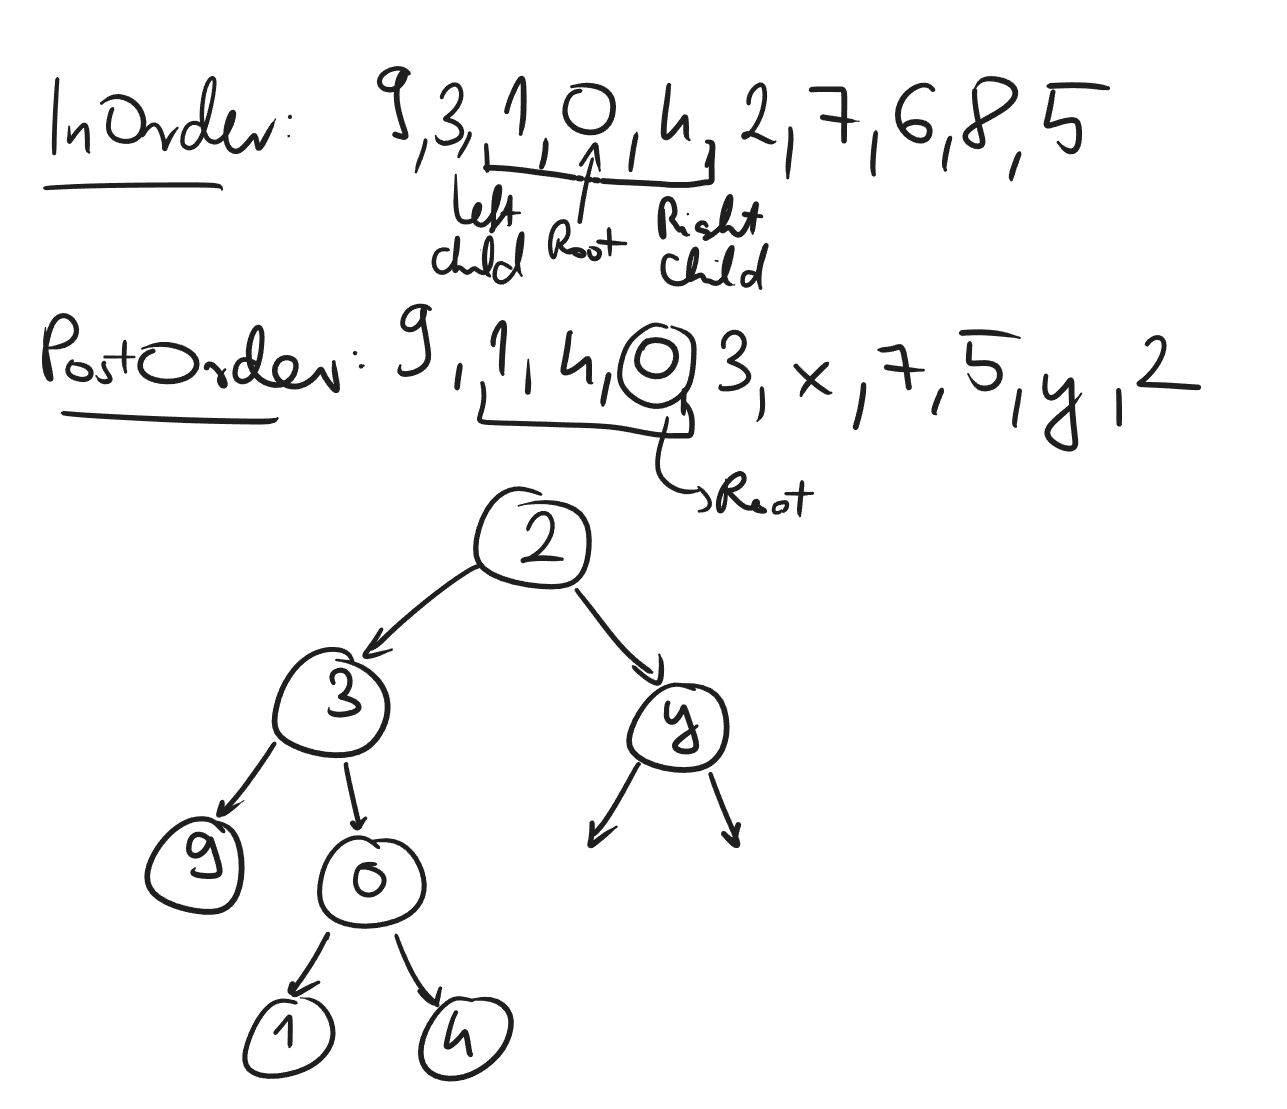
\includegraphics[width=\linewidth]{11/11/reconstruct_05.png}
\end{center}

\begin{itemize}
    \item Looking at the subtree $1,0,4$ in the PostOrder walk, we see that the last element is $0$, so that will be the root of that subtree.
    \item Then looking back at the InOrderWalk, we see that the left child must be $1$ (on the left of the root), while the right child must be $4$ (on the right of the root).
    \item We have reconstructed the left side of the root of the original tree.
    \item Now we need to think about the right side. $y$ could either be $6$ or $8$.
    \item Let's try $y=6$ and $x=8$.
\end{itemize}

\begin{center}
    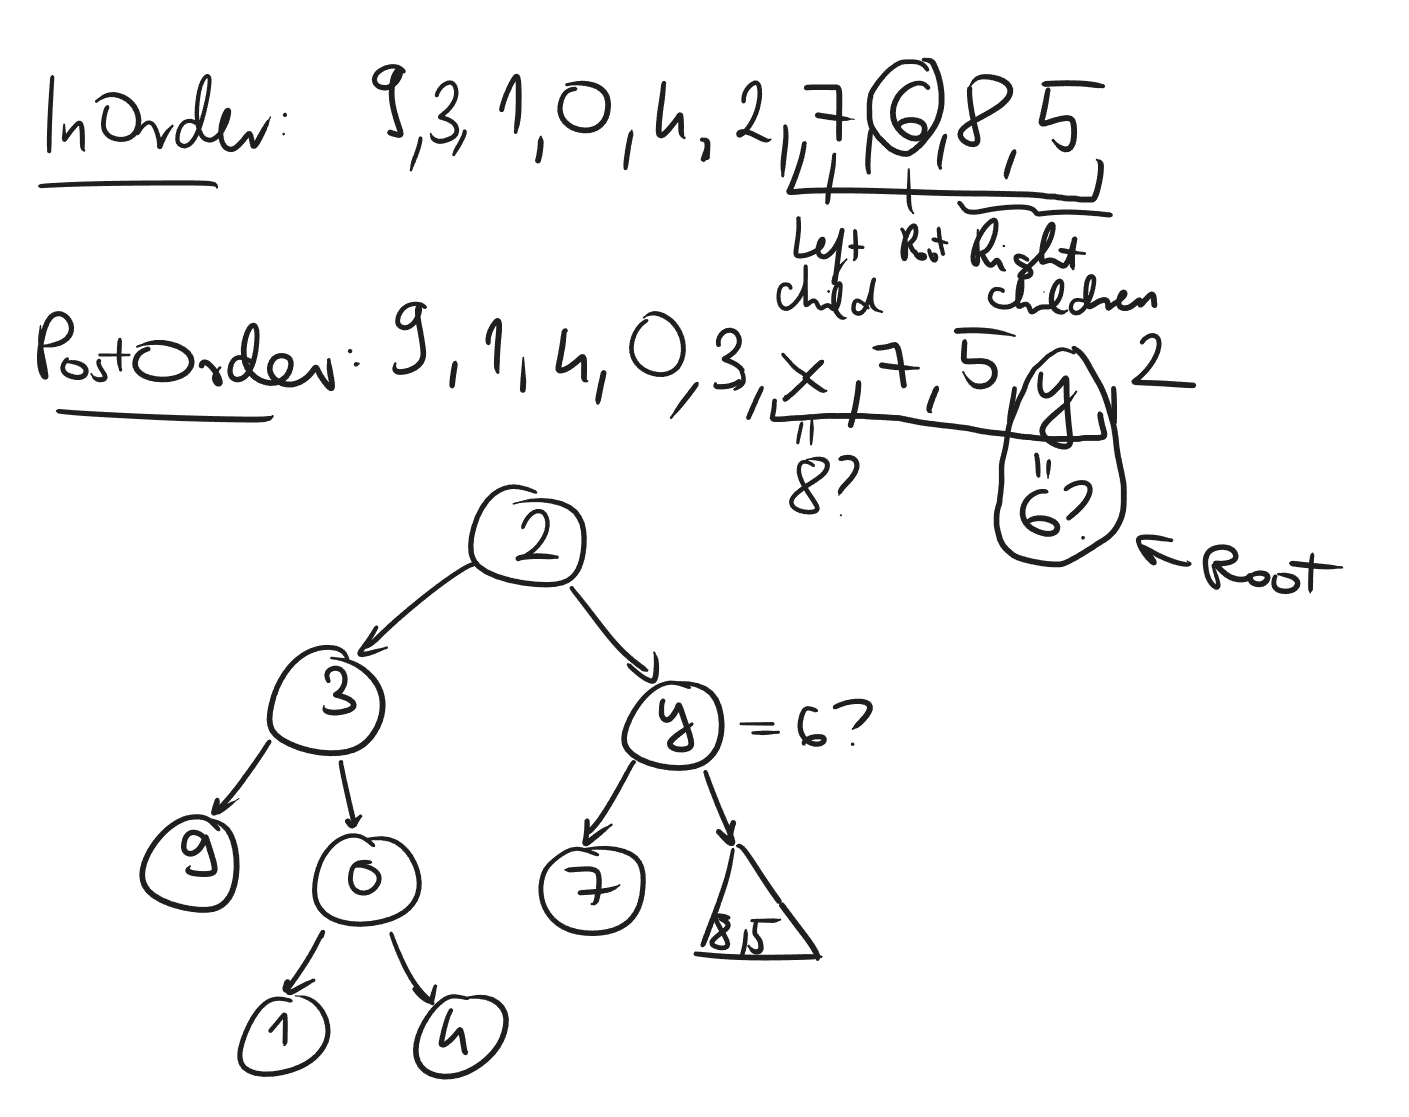
\includegraphics[width=\linewidth]{11/11/reconstruct_06.png}
\end{center}

\begin{itemize}
    \item Then we can step further, the $7$ must be the left child of $y=6$ and $x=8$ and $5$ must be on the right.
\end{itemize}

\begin{center}
    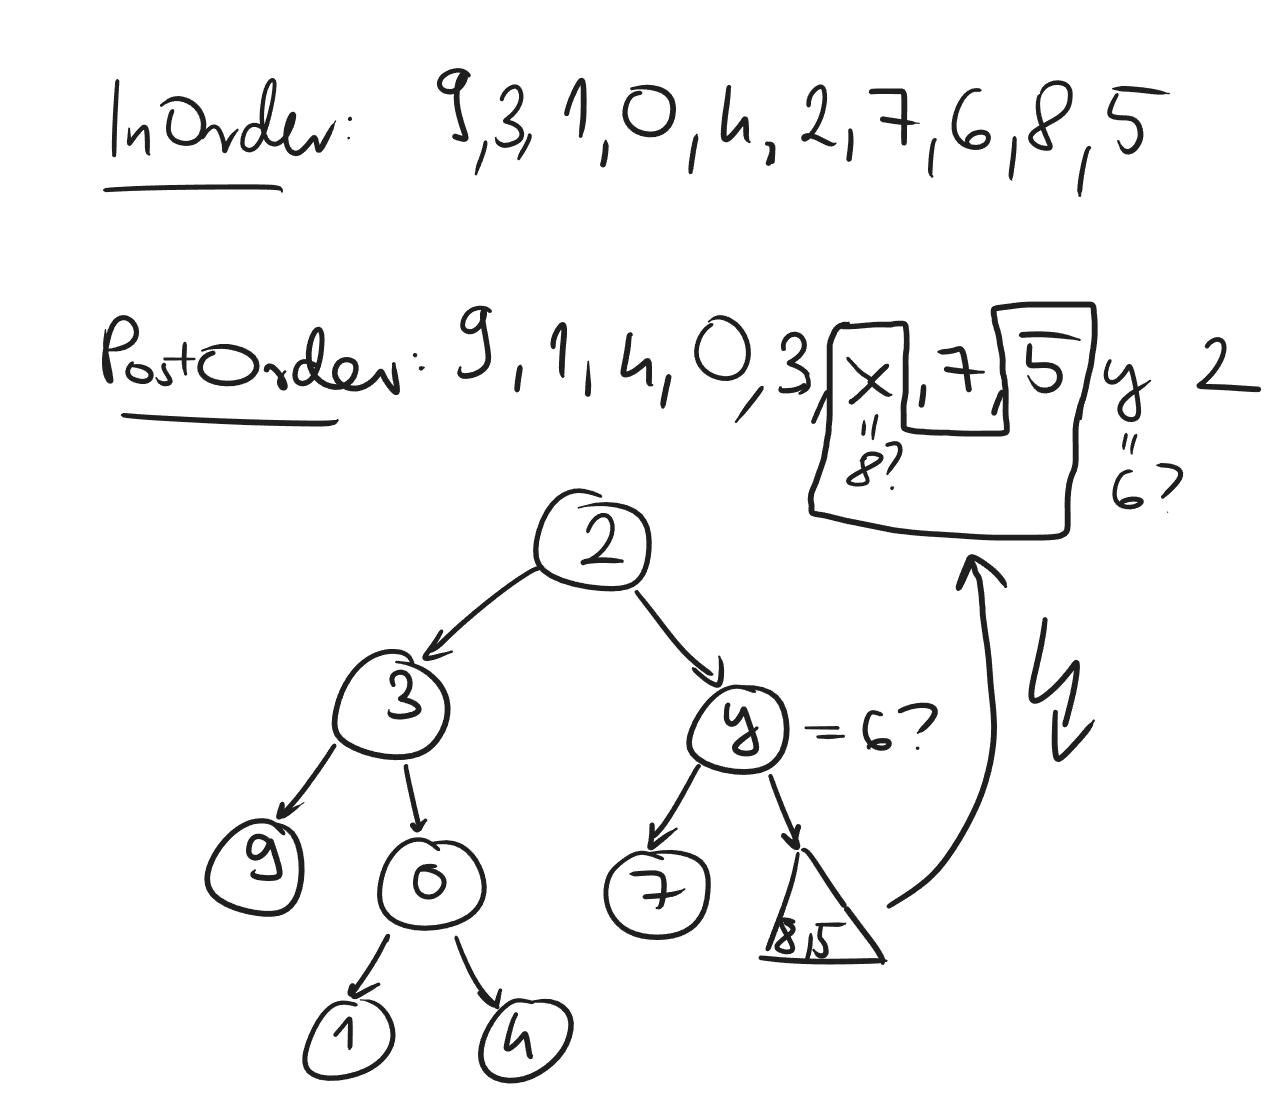
\includegraphics[width=\linewidth]{11/11/reconstruct_07.png}
\end{center}

\begin{itemize}
    \item However, this will result in a problem: $x=8$ and $5$ are a subtree, but in the PostOrder walk they appear not consecutively. Number $7$, which is their sibling subtree comes between them. This is impossible, subtrees should always appear in a consecutive order in all three of the walks! So this assignment cannot be correct!
    \item The only other way is $y=8$ and $x=6$, so let's go back and try doing that:
\end{itemize}

\begin{center}
    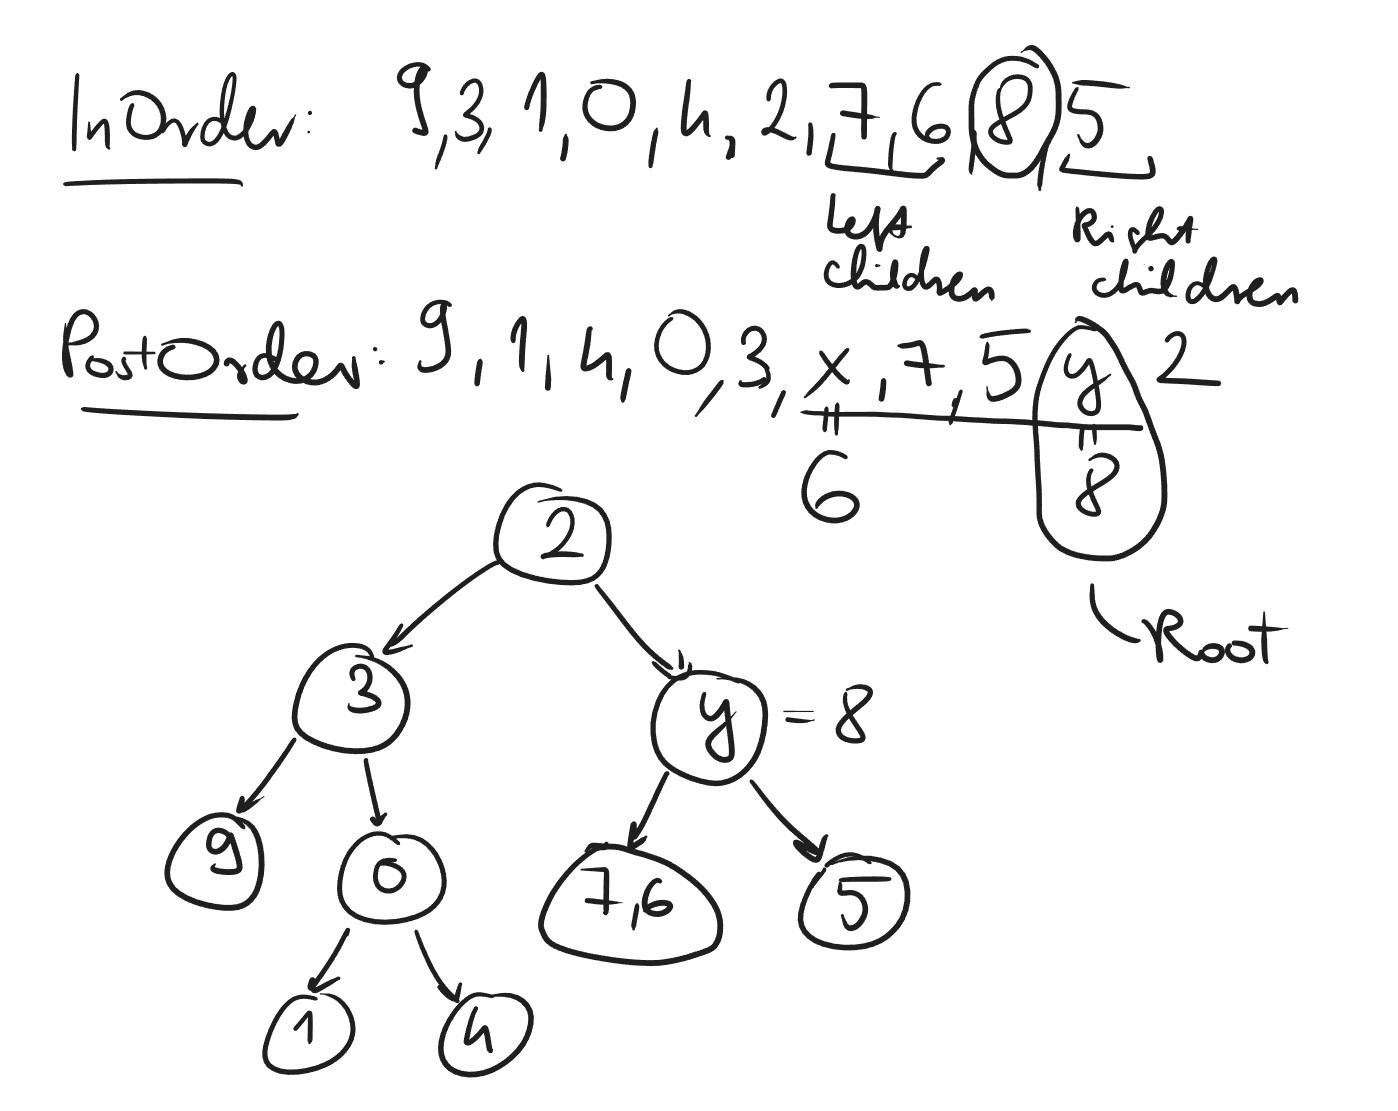
\includegraphics[width=\linewidth]{11/11/reconstruct_08.png}
\end{center}

\begin{itemize}
    \item Now we see that the left children of $y=8$ are $7$ and $6$, while the right child is $5$.
\end{itemize}


\begin{center}
    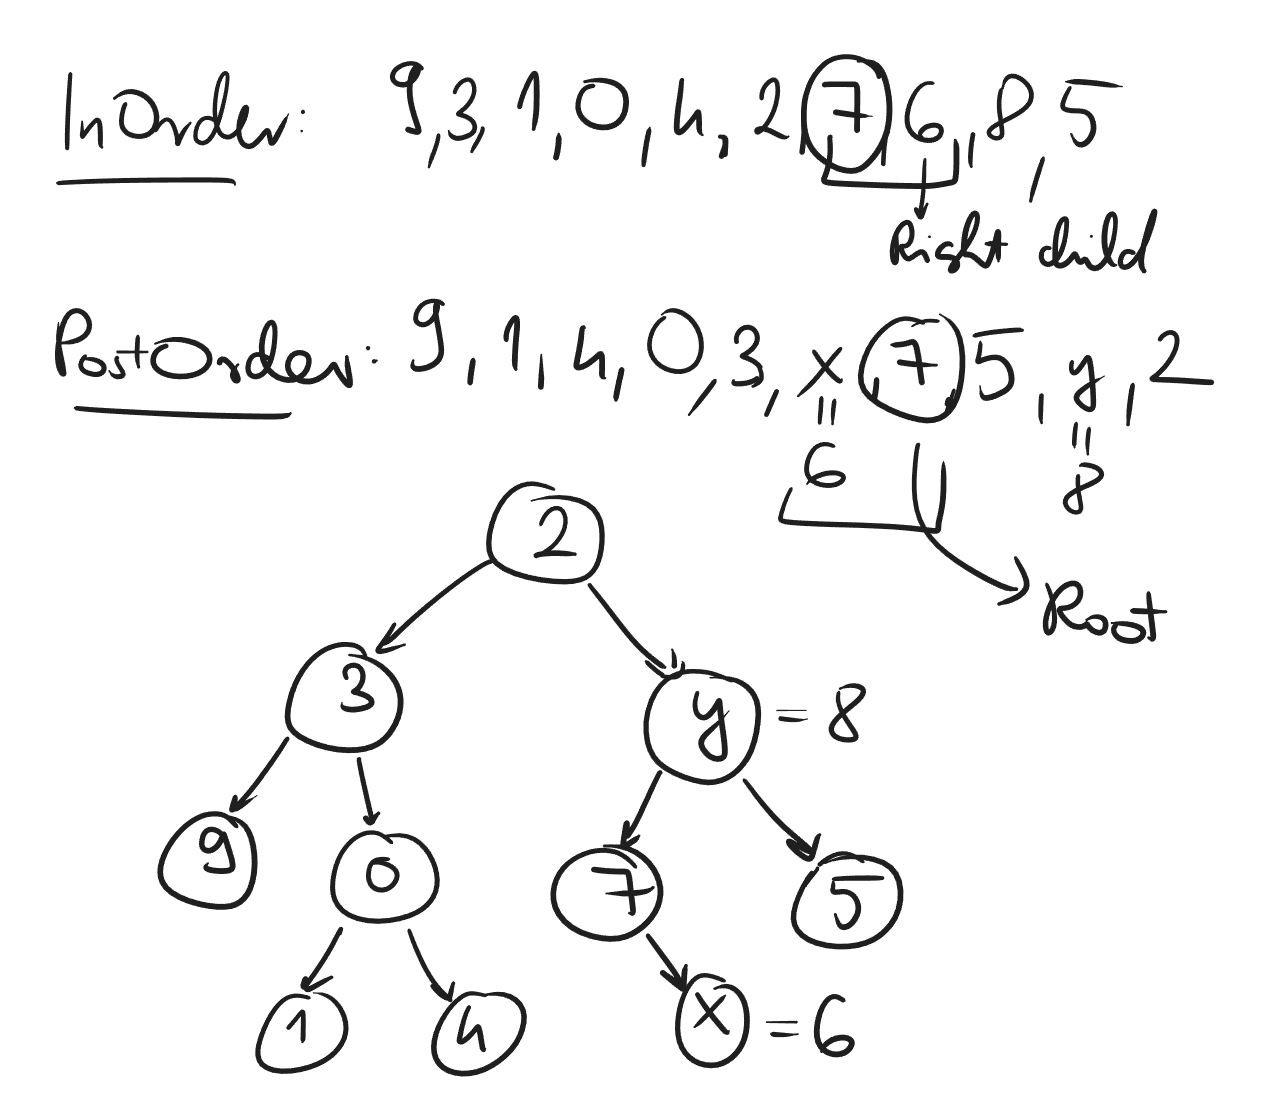
\includegraphics[width=\linewidth]{11/11/reconstruct_09.png}
\end{center}

\begin{itemize}
    \item This works well, since $7$ is the root of the $7,6$ subtree, we see this from the PostOrder result. Finally, $6$ is a right child of $7$, we see this from the InOrder walk.
    \item So $x=6$, $y=8$ and the corresponding tree is the one above.
\end{itemize}